\RequirePackage{ifvtex}
\documentclass[10pt,DIV17,a4paper,abstract=true,twoside=semi,openright]
{scrreprt}
\usepackage[T1]{fontenc}
\usepackage[utf8]{inputenc}
\usepackage{textcomp}
\bibliographystyle{abbrvnat}
\usepackage[english]{babel}
\RequirePackage[caption]{subfig}
\usepackage{isabelle}
\usepackage{isabellesym}
\usepackage{amsmath}
\usepackage{amssymb}
\usepackage[numbers, sort&compress, sectionbib]{natbib}
\usepackage{graphicx}
\usepackage{hyperref}
\usepackage{orcidlink}
\setcounter{tocdepth}{3} 
\hypersetup{%
   bookmarksdepth=3
  ,pdfpagelabels
  ,pageanchor=true
  ,bookmarksnumbered
  ,plainpages=false
} % more detailed digital TOC (aka bookmarks)
\sloppy
\allowdisplaybreaks[4]
\urlstyle{rm}
\isabellestyle{it}

% for uniform font size
%\renewcommand{\isastyle}{\isastyleminor}

\newenvironment{frontmatter}{}{}

\pagestyle{headings}
\isabellestyle{default}
\setcounter{tocdepth}{1}
\newcommand{\ie}{i.\,e.\xspace}
\newcommand{\eg}{e.\,g.\xspace}
\newcommand{\thy}{\isabellecontext}
\renewcommand{\isamarkupsection}[1]{%
  \begingroup% 
  \def\isacharunderscore{\textunderscore}%
  \section{#1 (\thy)}%
  \endgroup% 
}


\title{Isabelle/Solidity}
\subtitle{A deep Embedding of Solidity in Isabelle/HOL}
\author{Diego Marmsoler\textsuperscript{\orcidlink{0000-0003-2859-7673}}  
        and 
        Achim D. Brucker\textsuperscript{\orcidlink{0000-0002-6355-1200}}
		and Billy Thornton}%
\publishers{
Department of Computer Science, University of Exeter, Exeter, UK\texorpdfstring{\\}{, }
  \texttt{\{d.marmsoler, a.brucker, bt319\}@exeter.ac.uk}
}
\begin{document}
\begin{frontmatter}
\maketitle
\begin{abstract}
  \begin{quote}
    Smart contracts are automatically executed programs, usually representing
    legal agreements such as financial transactions. Thus, bugs in smart
    contracts can lead to large financial losses. For example, an incorrectly
    initialized contract was the root cause of the Parity Wallet bug that saw
    \$280M worth of Ether destroyed. Ether is the cryptocurrency of the
    Ethereum blockchain that uses Solidity for expressing smart contracts.

    We address this problem by formalizing an executable denotational semantics
    for Solidity in the interactive theorem prover Isabelle/HOL.  This formal
    semantics builds the foundation of an interactive program verification
    environment for Solidity programs and allows for inspecting them by
    (symbolic) execution. We combine the latter with grammar based fuzzing to
    ensure that our formal semantics complies to the Solidity implementation on
    the Ethereum blockchain.  Finally, we demonstrate the formal verification of
    Solidity programs by two examples: constant folding and a simple verified
    token.

      \bigskip
      \noindent\textbf{Keywords:} {Solidity, Denotational Semantics,
          Isabelle/HOL, Gas} 
  \end{quote}
\end{abstract}

\tableofcontents
\cleardoublepage
\end{frontmatter}


\chapter{Introduction}
An increasing number of businesses is adopting blockchain-based solutions. Most
notably, the market value of Bitcoin, most likely the first and most well-known
blockchain-based cryptocurrency, passed USD 1 trillion in February
2021~\cite{coinmarket}. While Bitcoin might be the most well-known application
of a blockchain, it lacks features that applications outside cryptocurrencies
require and that make blockchain solutions attractive to businesses.

For example, the Ethereum blockchain~\cite{Wood2014} is a feature-rich
distributed computing platform that provides not only a cryptocurrency, called
\emph{Ether}: Ethereum also provides an immutable distributed data structure
(the \emph{blockchain}) on which distributed programs, called \emph{smart
contracts}, can be executed. Essentially, smart contracts are automatically
executed programs, usually representing a legal agreement, e.g., financial
transactions. To support those applications, Ethereum provides a dedicated
account data structure on its blockchain that smart contracts can modify, i.e.,
transferring Ether between accounts. Thus, bugs in smart contracts can lead to
large financial losses.  For example, an incorrectly initialized contract was
the root cause of the Parity Wallet bug that saw \$280M worth of Ether
destroyed~\cite{perez.ea:smart:2021}. This risk of bugs being costly is already
a big motivation for using formal verification techniques to minimize this risk.
The fact that smart contracts are deployed on the blockchain immutably, i.e.,
they cannot be updated or removed easily, makes it even more important to ``get
smart contracts'' right, before they are deployed on a blockchain for the very
first time. 

For implementing smart contracts, Ethereum provides
\emph{Solidity}~\cite{Solidity}, a Turing-complete, statically typed programming
language that has been designed to look familiar to people knowing Java, C, or
JavaScript.  Notably, the type system provides, e.g., numerous integer types of
different sizes (e.g., \texttt{uint256}) and Solidity also relies on different
types of stores. While Solidity is Turing-complete, the execution of Solidity
programs is guaranteed to terminate. The reason for this is that executing
Solidity operations costs \emph{gas}, a tradable commodity on the Ethereum
blockchain. Gas does cost Ether and hence, programmers of smart contracts have
an incentive to write highly optimized contracts whose execution consumes as
little gas as possible. For example, the size of the integer types used can
impact the amount of gas required for executing a contract.  This desire for
highly optimized contracts can conflict with the desire to write correct
contracts.

In this paper, we address the problem of developing smart contracts in Solidity
that are correct: we present an executable denotational semantics for Solidity
in the interactive theorem prover Isabelle/HOL.

In particular, our semantics supports the following features of Solidity:
\begin{itemize}
	\item \emph{Fixed-size integer types} of various lengths and corresponding arithmetic.
	\item \emph{Domain-specific primitives}, such as money transfer or balance queries.
	\item \emph{Different types of stores}, such as storage, memory, and stack.
	\item \emph{Complex data types}, such as hash-maps and arrays.
	\item \emph{Assignments with different semantics}, depending on data types.
	\item An extendable \emph{gas model}.
	\item \emph{Internal and external method calls}.
\end{itemize}

A more abstract description of the semantics is given
in~\cite{marmsoler.ea:solidity-semantics:2021} and the conformance testing
approach for ensuring that our semantics conforms to the actual 
implementation is described in~\cite{marmsoler.ea:conformance:2022}.


The rest of this document is automatically generated from the formalization in
Isabelle/HOL, i.e., all content is checked by Isabelle. The structure follows
the theory dependencies (see \autoref{fig:session-graph}).

\begin{figure}
  \centering
  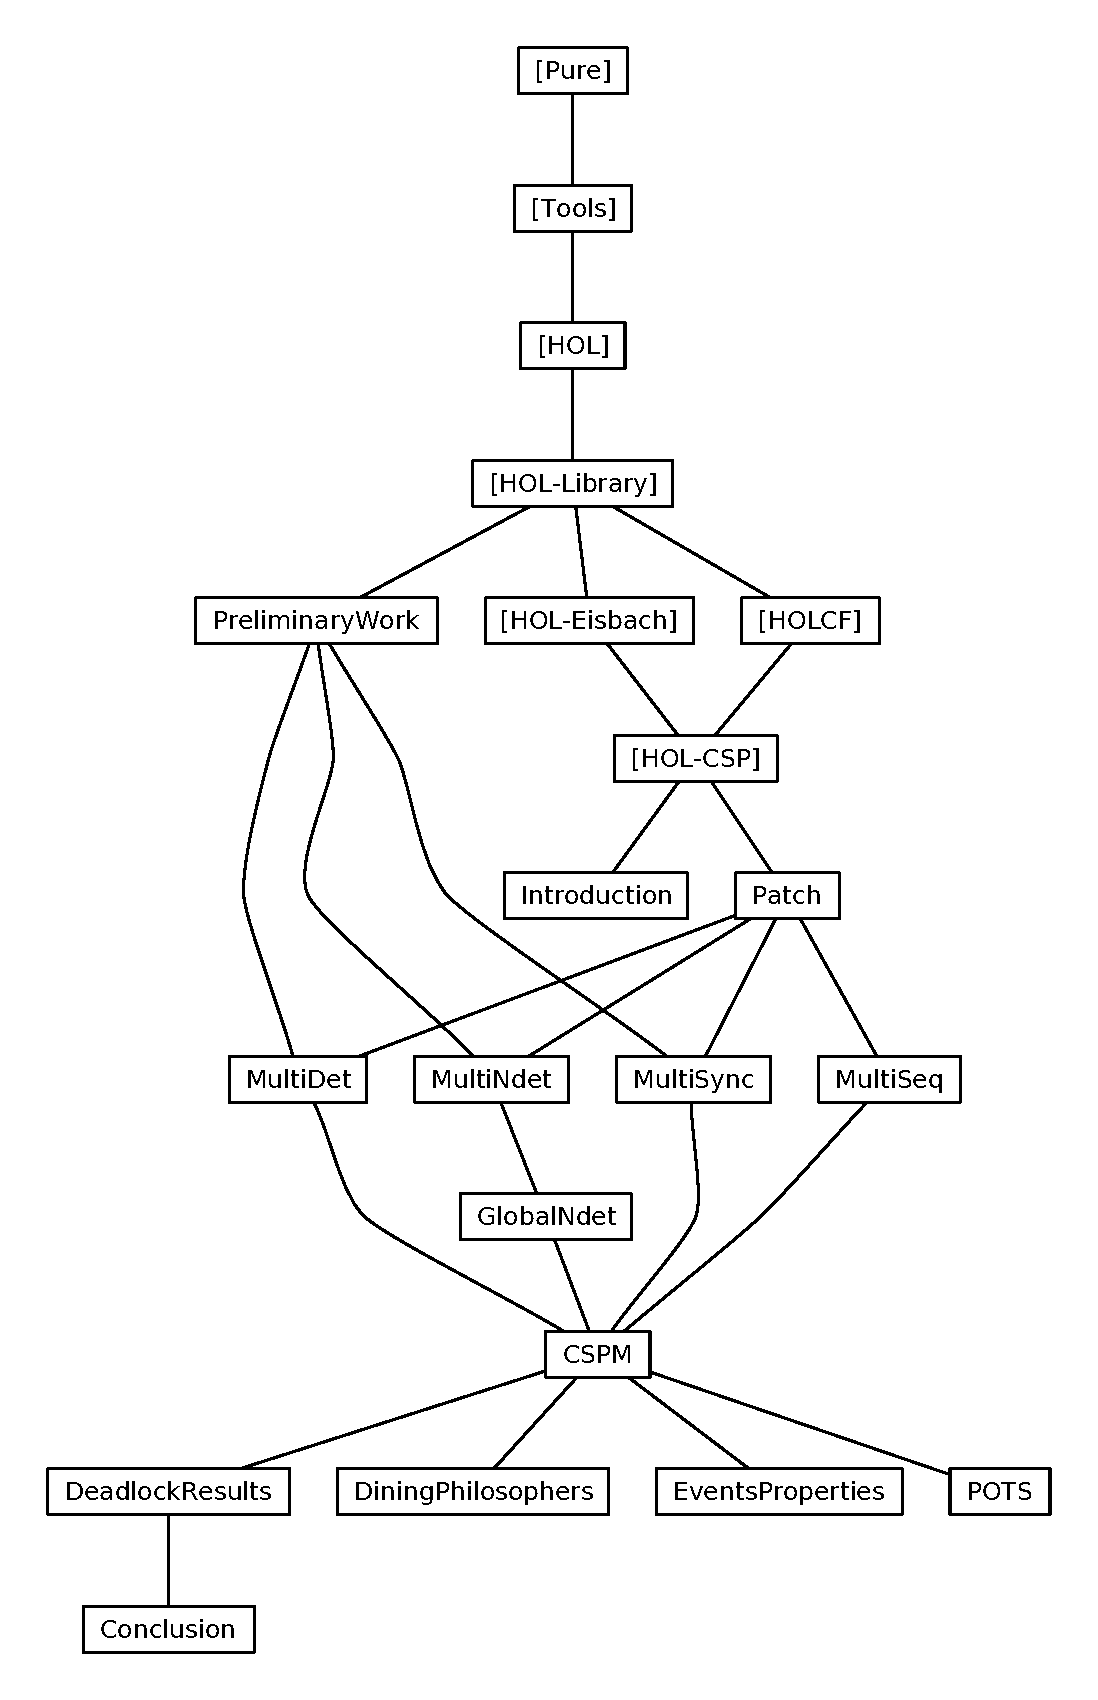
\includegraphics[height=.9\textheight, width=\textwidth,keepaspectratio]{session_graph}
  \caption{The Dependency Graph of the Isabelle Theories.\label{fig:session-graph}}
\end{figure}

\clearpage
%\input{session}

\chapter{Preliminaries}
In this chapter, we discuss auxiliary formalizations and functions that
are used in our Solidity semantics but are more generic, i.e., not
specific to Solidity. This includes, for example, functions to convert
values of basic types to/from strings.

\input{ReadShow.tex}
\input{Utils}
\input{StateMonad.tex}

\chapter{Types and Accounts}
In this chapter, we discuss the basic data types of Solidity and the
representations of accounts. 

\input{Valuetypes.tex}
\input{Accounts}

\chapter{Stores and Environment}
In this chapter, we focus on a particular aspect of Solidity that is
different to most programming languages: the handling of memory in
general and, in particular, the different between store and storage.

\input{Storage.tex}
\input{Environment.tex}

\chapter{Expressions and Statements}

In this chapter, we formalize expressions, declarations, and
statements. The results up to here form the core of our Solidity
semantics. 

\input{Contracts.tex}
\input{Expressions.tex}
\input{Statements.tex}
\input{Solidity_Main.tex}

\chapter{A Solidity Evaluation System}
This chapter discussed a tactic for symbolically executing Solidity statements
and expressions as well as provides a configuration for Isabelle's code
generator that allows us to generate an efficient implementation of our
executable formal semantics in, e.g., Haskell, SML, or Scala. In our test
framework, we use Haskell as a target language.
\input{Solidity_Symbex.tex}
\input{Solidity_Evaluator.tex}
\IfFileExists{Compile_Evaluator.tex}{%
    \input{Compile_Evaluator.tex}
}{}

\chapter{Verification Support}
This chapter presents a weakest precondition calculus and corresponding verification condition generator.

\input{Weakest_Precondition.tex}

\chapter{Applications}
In this chapter, we discuss various applications of our Solidity
semantics.

\input{Reentrancy}
\input{Constant_Folding.tex}

\IfFileExists{root.bib}{%
    \bibliography{root}
}{}
\end{document}

%%% Local Variables:
%%% mode: latex
%%% TeX-master: t
%%% End:
